
\renewcommand{\cleardoublepage}{}
\renewcommand{\clearpage}{}

\chapter{The Standard Model of Particle Physics}
\label{Chap:SM}

%\section{The Standard Model of Particle Physics}
%
%To pave the way for our future studies we present the SM. Complete with a overview of it's mechanisms and a brief historical introduction.
%
%\section{Motivation}

% { \color{red} Note! The motivation should explain why we are going indepth into flavour, and the Yukawa sector. There has to be a purpose to this section! } 

As stated in chapter \ref{Chap:Introduction}, it is hard to question the validity of the SM as a successful, at least approximate, framework, with whom to describe the phenomenology of particle physics up to the largest energy scales probed by collider measurements so far, although some inconsistencies remain and must be addressed.  
%
Note, what we call the SM is the conjugation of several theories, quantum chromodynamics (QCD), Higgs sector and the EW theory. 
%
% The last piece, the EW theory, was introduced in the nineteen sixties by Glashow, Salam and Weinberg \cite{SALAM1964168}, since then it has been extensively tested both in contemporary direct searches for new physics and indirect probes via e.g. flavour anomalies a\cite{Gr_newald_2008}. It awarded the authors the 1979 Noble prize of physics \cite{NobelPrize:2009-Physics}.  
%
%B. %, { \color{gray} and as said, it's been consistent with most to date.} 

The formulation of the SM came from previous principles relating to symmetries in nature, specifically symmetry in physical laws. 
%
In fact, much in modern physics can be attributed to Emmy Noether's work. She deduced, trough her first theorem, that if the action in a system is invariant under some group of transformations (symmetry), then there exist one or more conserved quantities (constants of motion) \cite{doi:10.1080/00411457108231446}. 

Physicists took this idea and were led to a fundamental question, is it possible that upon imposing to a given Lagrangian the invariance under a certain group of symmetries to reach a given form for its the dynamics? 
%
%These dynamics would be in our context, particle interactions. This train of thought first led to Quantum Electrodynamics (QED), then Quantum Chromodynamics (QCD) and finally the SM. 
%
We can quote Salam and Ward in Ref \cite{Salam1961}: % A. Salam and J. C. Ward, Nuovo Cim.19, 165 (1961). 

\textit{“Our basic postulate is that it should be possible to generate strong,  weak and electromagnetic  interaction terms (with all their correct symmetry properties and also with clues regarding their relative strengths) by making local gauge transformations on the kinetic energy terms in the free Lagrangian for all particles.”} % { \color{red} Question Morais: Is this really relevant I like it but it might be excess }

Although we are glossing over a lot of complexity in this statement, given that for the SM to be properly formulated, additional concepts are required. 
%
As in the case of weak interactions, the presence of a massive weak gauge boson requires the concept of spontaneous breakdown of the gauge symmetry via what is known as the Higgs mechanism \cite{higgs1964broken}. 
%
While the concept of asymptotic freedom played a crucial role in describing perturbatively the strong interaction at short distances \cite{politzer1973reliable}.  

\section{Internal symmetry of the Standard Model}
%
The SM is a gauge Quantum Field Theory (QFT), that is, manifestly invariant under a set of field transformations. The SM gauge group \cite{Quigg:1983gw}, $\mathcal{G}_{SM}$,% is seen in Eq. \ref{eq:SM_Group} . 
%
%The SM is manifestly invariant under of a set of field transformations. The SM is a gauge group \cite{Quigg:1983gw}, $\mathcal{G}_{SM}$, is seen in, 
%
\begin{equation}
\mathcal{G}_{SM} = \mathrm{SU}(3)_{\mathrm{C}} \times \SU{L} \times \U{Y}   .
\label{eq:SM_Group}
\end{equation} 
%
Where, $\mathrm{SU}(3)_{\mathrm{C}}$, with $\mathrm{C}$ being colour, is the group that describes the QCD sector, responsible for the strong force. This symmetry will remain unbroken by the EW Vacuum Expectation Value (VEV).
%
Secondly, we have the $\SU{L} \times \U{Y}$ portion, with L being Left and Y the hypercharge, that will be broken by the Higgs mechanism into $\U{Q}$, the electromagnetic gauge symmetry.

Each particle in the SM stems from a field that is charged in a particular manner on each of these groups.  
%
Recall that Quantum Field Theory (QFT) treats particles as excited states of their respective quantum fields, which are more fundamental than the particles. 
%
Interactions between particles are described by interaction terms in the Lagrangian involving their corresponding quantum fields.
%
Of which each interaction can be visually represented by a Feynman diagram according to perturbation theory.
%
Generally speaking, an interacting QFT can not be solved analytically, requiring the use of perturbative methods. 
%
In this mindset, one employs the use of Feynman diagrams to better visualize interactions at any given order in perturbation theory.

It is important to highlight that given the invariance under the group in Eq.\,(\ref{eq:SM_Group}), it is impossible for any field, besides the scalar field, to have an explicit mass term in the bare Lagrangian.
%
In this chapter we shall present how the mass of particles is generated via the Higgs mechanism.
%
And offer a brief discussion of flavor physics in the SM and how flavor changing currents can point to NP. 

%{ \color{gray} All masses for the fermions and leptons are generated trough their interactions with the Higgs Boson. This mass generation as the Higgs Boson settles into it's VEV is called the Higgs Mechanism. } 

\subsubsection{Particle States and Fields}

The particle spectrum of the SM is composed by, the gauge bosons, $W^\pm$ and $Z$ bosons, mediators of the weak interactions, the photon $\gamma$, the electromagnetic interaction messenger and the strong force mediators, the gluons, $G$. 
%
Additionally, the model is also composed  by the matter particles, the fermions, composed by quarks and leptons. A spin-0 scalar also emerges known as the Higgs Boson, $h$. 

Leptons and quarks are organized in three generations each, with 2 pairs by each generation leading to 6 different particles. 
%
For quarks we have the up and down for the first generation, charm and strange for the second as well as the top and bottom for the third one. 
%
Similarly, there are 6 types of leptons, the 3 charged leptons, electron, muon and tau, and the associated neutrinos. 
%
These are represented in different manners, being that the quarks are represented by $(u,d,c,s,t,b)$ while leptons as $(e,\nu_{e},\mu,\nu_{\mu},\tau,\nu_{\tau})$, where $\nu$ denotes the neutrinos. 

%Fermions are half integer spin particles where half of which have electrical charge (except the neutrinos).  
%
While quarks interact via the weak, electromagnetic and strong forces, the charged leptons only feel the electromagnetic and weak forces and the neutrinos are weakly interacting.  
%
A physical fermion is composed of a left-handed and a right-handed field. The left-handed components of the fermions are doublets under $\mathrm{SU(2)}_L$, 
%
\begin{equation}
L^i= \begin{pmatrix}
\nu_{e_L} \\ e_L 
\end{pmatrix},
\begin{pmatrix}
\nu_{\mu_L} \\ \mu_L 
\end{pmatrix},
\begin{pmatrix}
\nu_{\tau_L} \\ \tau_L 
\end{pmatrix} 
\quad 
\text{and} \quad Q^i= \begin{pmatrix}
u_{L} \\
d_L 
\end{pmatrix},\begin{pmatrix}
c_{L} \\
s_L 
\end{pmatrix}
,\begin{pmatrix}
t_{L} \\
b_L 
\end{pmatrix} ,
\end{equation}
%
where the $i$ index stands for generation, often designed as the flavour index. Conversely the right-handed components are singlets of  $\SU{L}$ and are represented as,
%
 \begin{equation}
e^i_R=\{e_R,\mu_R,\tau_R\}, \quad  u^i_R=\{u_R,c_R,t_R\}, \quad d^i_R=\{d_{R},s_{R},b_{R}\} . 
\end{equation}
%
Note also that the quarks form triplets of $\mathrm{SU(3)_C}$ whereas leptons are color singlets, meaning that only quarks interact strongly. 
%
The Higgs boson also emerges from an $\mathrm{SU(2)_L}$ doublet with the form,
%
\begin{equation}
H=\begin{pmatrix}
\phi^1 + \; i \; \phi^2 \\
\phi^3 + \; i \; \phi^4  
\end{pmatrix} \equiv \begin{pmatrix}
\phi^+ \\
\phi^0 
\end{pmatrix}, 
\end{equation}
%
%The Lagrangian that describes all vector particles and gauge fields in the SM can be writen as
%
where we see the four components that correspond to the respective degrees of freedom of the Higgs Field.
% 
After the process of Spontaneous Symmetry Breaking (SSB) of the $\mathrm{SU(2)_L} \times \U{Y}$ group, the charges read as,
%
\begin{table}[H]
\caption{Quark and Lepton charges}
\centering
\begin{tabular}{ccc}
  \hline & $\mathrm{SU(3)_C}$ & $\mathrm{U(1)_Q}$ \\
  \hline 
Up type quarks $(u,c,t)$ & \textbf{3} & 2/3 \\
Down type quarks $(d,s,b)$ & \textbf{3} & -1/3 \\
Charged leptons $(e,\mu,\tau)$ & \textbf{1} & -1 \\
Neutrinos  $(\nu_e,\nu_\mu,\nu_\tau)$  & \textbf{1} & 0 \\
  \hline	
\end{tabular}
\end{table}


\subsubsection{Gauge Group Numbers}

The full set of SM fields and respective quantum numbers are are shown in the tables \ref{table1} and \ref{table2}. These show us the representations of these fields, e.g. if a field $F$ has a quantum number of 3 under $\mathrm{SU(2)_L}$ then he would be a triplet of of $\mathrm{SU(2)_L}$, \ $F^a = (F^1,F^2,F^3)$, where $a$ is an index in the adjoint representation of the group.   
%
\begin{table}[H]
\centering
\caption{Gauge and Scalar fields in the SM}
\label{table1}
\begin{tabular}{@{}cccccc@{}}
  \hline	
 Fields & Spin 0 field & Spin 1 Field & $ \mathrm{ SU(3)_C \times SU(2)_L \times U(1)_Y } $  \\
  \hline	
 Gluons  & $\times$  & $G^a$ & (\textbf{8},\textbf{1},0) \\	
A bosons & $\times$  & $A^a$ & (\textbf{1},\textbf{3},0)   \\
B bosons & $\times$  & $B$   & (\textbf{1},\textbf{1},0)   \\
Higgs field & ($\phi^\pm, \phi^0 )$  & $\times$ & (\textbf{1},\textbf{2},1) \\ \hline
\end{tabular}
\end{table}
%
The gauge groups presented in table \ref{table1} are composed of 12 generators and are governed by the following algebra, 
% 
\begin{equation}
\left[ M_a , M_b \right] = i f_{abc} M_c \quad \left[ T_a , T_b \right ] = i \epsilon_{abc} T_c \quad \left[ M_a , T_b \right] = \left[ M_a , Y \right] = \left[ T_b,Y \right] = 0  \ , 
\end{equation}
%
where for $\mathrm{SU(3)_c}$, $M_a = {\lambda_a}/{2}$ , with $(a = 1, . . . , 8)$. As for $\mathrm{SU(2)_L}$, we have $T_i= \sigma_i/{2} $, $(i = 1, 2, 3)$, and for $Y$ is the generator of $U(1)_Y$. The symbols $\lambda_a$ and $\sigma_i$ represent the Gell-Mann and Pauli matrices respectively. 
%
\begin{table}[H]
\centering
\caption{Fermion fields in the SM}
\label{table2}
\begin{tabular}{@{}cccccc@{}}
  \hline	
 Fields & Spin $\frac{1}{2}$ Field & $\mathrm{ SU(3)_C \times SU(2)_L \times U(1)_Y} $   \\
  \hline	
Quarks (3 gen.) & $Q=(u_L,d_L)$ & $(\mathbf{3},\mathbf{2},{1}/{3})$ \\	
$\quad$        & $u_R$ & $(\mathbf{3},\mathbf{1},{4}/{3})$   \\
$\quad$   & $d_R$ & $(\mathbf{3},\mathbf{1}, -{2}/{3})$   \\
Leptons (3 gen.) & $L=(\nu_{e_L}, e_L )$ & $(\mathbf{1},\mathbf{2},-1)$  \\
$\quad$   & $e_R$ & $(\mathbf{1},\mathbf{1},-2)   $ \\ \hline
%
\end{tabular}
\end{table}
%
From here, given the gauge group in, Eq.\,(\ref{eq:SM_Group}) and accounting for the charges and fields, we can derive the form of the SM's Lagrangian. 



%\subsection{Fields, Particles and Lagrangian of the SM}

\subsubsection{Lagrangian Formulation }
%
Given the SM gauge groups seen in  Eq.\,(\ref{eq:SM_Group}), the charges seen in Tables \ref{table1} and \ref{table2} and their algebra, the covariant derivative, $D_\mu$, can be shown to read as, 
%
\begin{equation}
\label{eq:PartialDefSM}
D_\mu = \partial_\mu - i g_s M^a G^a_\mu - i g T^i A^i_\mu - \frac{1}{2} i g' Y B_\mu \quad ,  
\end{equation}  
%
We can expect 3 different type of couplings, $g_s$ related to the $\mathrm{SU(3)_C}$ subgroup, $g$ to the $\mathrm{SU(2)_L}$ and $g^\prime$ to $\mathrm{U(1)_Y}$. The associated canonical field strength tensors would be,
\begin{align}
G_a^{\mu \nu} & = \partial^\mu G^\nu_a - \partial G^\mu_a - g_s f_{abc} G_a^\mu G_b^\nu ,  \\ 
A_a^{\mu \nu} & = \partial^\mu A^\nu_a - \partial^\nu A^\mu_a  - g  \epsilon_{abc} A^\mu_b A^\nu_c , \\
B^{\mu \nu}   & = \partial^\mu B^\nu - \partial^\nu B^\mu .
\end{align}
%
Given these we can now present the SM Lagrangian. It is often convenient to do so in portions, usually divided in three \footnote{There is also the need for the introduction of gauge fixing terms and ghosts. However, this is merely a formal requirement and does not imply addition of new physical states.} sections,
\begin{equation}
\mathcal{L}_{SM} = \mathcal{L}_{kin}  +  \mathcal{L}_{Yuk} +  \mathcal{L}_{\phi} , 
\end{equation}
Where we have the kinetic portion of the SM terms, $\mathcal{L}_{kin}$, responsible for  free propagation of particles, the Yukawa portion, $\mathcal{L}_{Yuk}$,  corresponding to interactions of particles with the Higgs Boson, and finally the $\mathcal{L}_{\phi}$ scalar potential. The full kinetic portion of the SM read, 
%
\begin{align}
\label{eq:KinSM}
\mathcal{L}_{kin} = & - \frac{1}{4} G^{\mu \nu}_a G_{a \, \mu \nu}  - \frac{1}{4}  A^{\mu \nu}_a A_{a \,\mu \nu}  
- \frac{1}{4}  B^{\mu \nu} B_{\mu \nu} \nonumber \\ 
 & -i \bar{Q}_{L_i} \slashed{D} Q_{L_i} 
   -i \bar{u}_{R_i} \slashed{D} u_{R_i}  
   -i \bar{d}_{R_i} \slashed{D} d_{R_i}  
   -i \bar{L}_{L_i} \slashed{D} L_{L_i}    
   -i \bar{e}_{R_i} \slashed{D} e_{R_i}   \\
 & - (D_\mu H)^\dagger ( D^\mu H ) ,  \nonumber 
\end{align}
where $\slashed{D}$ is the Dirac covariant derivative, $\gamma^\mu D_\mu$ where $\gamma^\mu$ being the gamma matrices. 
%
From the last line of Eq.\,(\ref{eq:KinSM}) and with Eq.\,(\ref{eq:PartialDefSM}) we will present how the fields $A^a_\mu$ and $B_\mu$ give rise to the weakly interacting vector bosons $W^\pm$ and $Z^0$ and the electromagnetic vector boson $\gamma$. Contrary to the colour sector, where the eight generators $G^a_\mu$ simply correspond to eight gluons $G$ mediating the strong interactions.
%
The scalar potential part is written as, 
%
\begin{equation}
\label{eq:PotentialSM}
\mathcal{L}_{\phi} = -\mu^2 H H^\dagger - \lambda (H H^\dagger)^2 .
\end{equation}
%
Finally the Yukawa portion of the Lagrangian is, 
%
\begin{equation}
\label{eq:YukawaSM}
\mathcal{L}_{Yuk} = Y^u_{ij} \bar{Q}_{L_i} u_{R_j}  \tilde{H} + Y^d_{ij} \bar{Q}_{L_i}  d_{R_j} H  + Y^e_ij \bar{L}_{L_i}  e_{R_i} H + \text{H.c.} \ ,
\end{equation}
%
where, $\tilde{H}=i\sigma_2 H$ and H.c. stands for Hermitian conjugate, also the terms $Y^{e,u,d}$ stands for the Yukawa matrices, these are generic $3\times3$ with complex and adimensional matrix elements. Note that all indices seen in Eqs.\,(\ref{eq:KinSM}), (\ref{eq:PotentialSM}) and (\ref{eq:YukawaSM}), ($j,i$) are summed over. 

%{ \color{red} Perguntar ao Morais : Remover o italico dos campos? } 
%
%{ \color{gray} It is due to the Yukawa interactions between the Higgs and the fermions and leptons that these acquire their masses once the Higgs settles into his VEV. } { \color{blue} same as before }
%
%We'll define these fields in the relevant section. Note that naturally all indices seem in Eqs. \ref{eq:KinSM} \ref{eq:PotentialSM} and \ref{eq:YukawaSM}, ($j,i$) are summed over. 


\renewcommand{\cleardoublepage}{}
\renewcommand{\clearpage}{}

\section{The Higgs Mechanism and the Mass Generation of the Gauge Bosons}

From what was defined above, we can now study the process SSB by which, 
%
\begin{equation}
\SU{L}\times\U{Y} \rightarrow \U{Q}. 
\end{equation} 
%
Enabling us to find the real physical states of the gauge bosons and the origin of their mass. Let us consider the part of the Lagrangian containing the scalar covariant derivatives, the scalar potential and the gauge-kinetic terms:
%
\begin{equation}
\mathcal{L}_{Gauge} \supset (D_\mu H)(D^\mu H)^\dagger - \mu^2 H^\dagger H - \lambda (H^\dagger H)^2 - \frac{1}{4}  W^{\mu \nu}_a W_{a \,\mu \nu}  
- \frac{1}{4}  B^{\mu \nu} B_{\mu \nu} \ . 
\label{eq:GaugeSM}
\end{equation} 
% 
We expect a phase shift to occur, namely one that ensures $\mu^2 < 0$ while at the same ensuring that the field now explicitly breaks the $\mathrm{SU(2)_L \times U(1)_Y}$. For this to happen we expect the shifted squared value of the Higgs field to be,
%
\begin{equation}
(H^\dagger H)^2 = \frac{-\mu^2}{2\lambda} \equiv  v^2  , 
\end{equation} 
called the EW-Vacuum expectation value (EW-VEV), its value is experimentally measured to be $v \approx 246$ GeV. 
%
The choice of vacuum can be aligned in such a way that we have,
\begin{equation}
H_{min} = \frac{1}{\sqrt{2}} \begin{pmatrix} 0 \\
v 
\end{pmatrix}  .
\end{equation}

Given that now the $\mathrm{SU}(2)_{\mathrm{L}} \times \mathrm{U}(1)_{\mathrm{Y}}$ symmetry is broken down to $U(1)_{\mathrm{Q}}$ we jump from a scenario where there were four generators, which are $T^{1,2,3}$ and $Y$, to, after the breaking, having solely one unbroken combination that is $Q =  (T^3 + Y/2)$ associated to the electric charge.
%
This means that in total we will have three broken generators, thus, from the Goldstone theorem, there would have to be created three massless particles. % { \color{red} Do I need citation? }

These Goldstones modes however can be parameterized as phases in field space and can be absorbed into the physical basis fields, leaving us with a single physical massive scalar, the Higgs boson. 
%
Note that, with this transformation we are removing three scalar degrees of freedom and transferring them to the gauge bosons.  %However, they cannot just disappear from the theory and will be absorbed by the massive gauge bosons.
%
%In fact, a massless gauge boson contains only two scalar degrees of freedom (transverse and polarization). Meanwhile, a massive vector boson has two transverse and a longitudinal polarization, i.e., three scalar degrees of freedom. 
%
So, while before the breaking of the EW symmetry we have four massless gauge bosons, after the breaking we are left with three massive ones.
%
%This means that there are three extra scalar degrees of freedom showing up in the gauge sector.
%
%It is then commonly said that the goldstone bosons are ``eaten" by the massive gauge bosons and the total number of scalar degrees of freedom in the theory is preserved. 
%
Therefore, without loss of generality, we can rewrite the Higgs doublet as
%
\begin{equation}
 \begin{pmatrix}
\phi_1 + i \phi_2 \\ 
v + h + i \phi_3 
\end{pmatrix} = H  \rightarrow H =  \frac{1}{\sqrt{2}} \begin{pmatrix}
0 \\ 
v + h 
\end{pmatrix}  .
\label{shame}
\end{equation}
Once the Higgs doublet shifts to the EW-VEV, the Lagrangian (\ref{eq:GaugeSM}) can be recast as:
%
\begin{align}
\mathcal{L}^\prime = & \frac{1}{2} \partial_\mu h \partial^\mu h - \frac{1}{2} (2v^2 \lambda) h^2
 - \frac{1}{4}  W^{\mu \nu}_a W_{a \, \mu \nu}  
- \frac{1}{4}  B^{\mu \nu} B_{\mu \nu}  \nonumber \\
& + \frac{1}{8} v^2 g^2 (A^1_\mu A^{1,\mu}+ A^2_\mu A^{2,\mu}) +  \frac{1}{8} v^2  (g^2  A^3_\mu A^{3,\mu} + g^{\prime 2} B_\mu B^\mu - 2 g^2 g^{\prime 2} A^3_\mu B^\mu )  \ , 
\label{complicatedpart}
\end{align}
%
A few things become obvious. First, we have a lot of mass terms stemming from the squared gauge fields and a lonesome mass term belonging to the real scalar field we know to be the Higgs field. This makes the Higgs boson mass to be given by,
%
\begin{equation}
M_h= (2v^2 \lambda).  
\end{equation}
%
To obtain masses for the gauge bosons we need to rotate the gauge fields to a basis where the mass terms are diagonal. First, it is straightforward to see that the electrically charged eigenstates are given by %\ref{gagestate}
%First the fields that carry defined charge that can be easily shown to be 
\begin{equation}
W^\pm_\mu = \frac{1}{\sqrt{2}} (A^{1}_\mu \pm i A^{2}_\mu) , 
\label{gagestate}
\end{equation}
meaning that the mass of the W bosons is, 
\begin{equation}
M_{W^\pm}= \frac{1}{2} v g .
\end{equation}
%
The situation becomes a bit more complicated for the second term in (\ref{complicatedpart}) due to a mixing between $A_\mu^3$ and $B_\mu$. In the gauge eigenbasis the mass terms read
%
\begin{equation}
\begin{pmatrix}
A_\mu^3 && B_\mu
\end{pmatrix} \cdot  \frac{1}{2} v^2 \begin{pmatrix}
g^2  & -g g^\prime \\
-g g^\prime & g^{\prime 2} 
\end{pmatrix} \cdot \begin{pmatrix}
A^{\mu,3} \\  B^\mu
\end{pmatrix}  , 
\end{equation} 
%
which can be diagonalized to obtain,
%
\begin{equation}
\begin{pmatrix}
A_\mu && Z_\mu 
\end{pmatrix} \begin{pmatrix}
0  & 0 \\
0  & \frac{1}{2} v \sqrt{g^2 + g^{\prime 2}} 
\end{pmatrix}  \begin{pmatrix}
A^\mu \\ Z^\mu
\end{pmatrix} , 
\end{equation}
%Where the new eigenvectors that represent the $Z$ boson and the photon, $A^\mu$ in terms of the former base are written as,
%
we identify the eigenvector associated with the null eigenvalue to be the photon and the massive one, $ M_Z =  \frac{1}{2} v \sqrt{g^2 + g^{\prime 2}} $, to be the Z boson. Such eigenvectors can be written as
%
\begin{align}
A_\mu &=\cos(\theta_W) B_\mu + \sin(\theta_W) A_\mu^3 ,  \\  
Z_\mu & =- \sin(\theta_W) B_\mu + \cos(\theta_W) A_\mu^3 , 
\end{align}
%
where $\theta_W$ is the so called Weinberg mixing angle and is defined as, 
%
\begin{equation}
\cos(\theta_W)=\frac{g}{ \sqrt{g^2 + g^{\prime 2}}} . 
\end{equation}
%
%{ \color{gray} Thus showing the massless photon along with a massive Z boson with mass $M_Z= \frac{1}{2} v \sqrt{g^2 + g^{\prime 2}} $ }. 
%
So we conclude our exploration of the electroweak sector with all the correct massive spectrum observed and its origin discussed.

\renewcommand{\cleardoublepage}{}
\renewcommand{\clearpage}{}

\section{Fermion Masses in the SM and Quark mixing}

As referenced \Joaoadd{previously}, given the charges of the fermion and lepton fields\Joaoadd{,} we cannot construct a gauge invariant theory with explicit mass terms for fermions. 
%
The mass of these particles \Joaorep{are generated through couplings to the Higgs, by the Higgs mechanism}{are generated through the Higgs mechanism, via Yukawa terms between the fermions and the scalar field. These interactions can be seen in Eq.\,\eqref{eq:YukawaSM}}. \Joaoout{We can write these interactions as,}
%
%\begin{equation} 
%\label{eq:Yukawa2}
%\mathcal{L}_{Yuk} = Y^u_{ij}\bar{Q}_{i} u_{R_j}  \tilde{H} + Y^d_{ij} \bar{Q}_{i}  d_{R_j} H  + Y^e_{ij} \overline{L_{L_i}}  e_{R_i} H + h.c.
%\end{equation} 
%
\Joaoout{where $Y^{e,u,d}$ stand for the Yukawa matrices, these are generic $3\times3$ complex non-dimensional coupling matrices, $H$ is the Higgs field with $\tilde{H}$ retaining it's previous definition, $i,j$ are the standard generation indices, $Q_{L_i}$,are the left handed quark doublets, while $d_R$ and $u_R$ are the corresponding right-handed down and up quark singlets respectively in the weak eigenstate basis.}
%
\Joaorep{Has}{As} the Higgs field settles into the electroweak VEV \Joaoadd{(see Eq.\,\eqref{eq:vev_expansion})} \Joaoout{yields} mass terms for the quarks and leptons \Joaoadd{are generated}. 
%
The Higgs mechanism generates the mass for all the fermionic and leptonic particles except for neutrinos\Joaoadd{. T}his is due to the SM not containing right handed neutrinos, i.e we \Joaorep{can't}{can not} build terms that would lead to neutrino masses.
% 
The addition of right handed neutrino fields is very commonly made in BSM scenarios. 

To reach the physical states \Joaoout{starting} from the weak eigenbasis \Joaorep{you}{we} must diagonali\Joaoadd{s}e the Yukawa matrices. This is done through \Joaoout{a} bi-unitary transformation\Joaoadd{s}. 
% 
We can write these transformation under the form,
%
\begin{equation}
\label{YukawaMasses} 
M^{u,d,e}_{\text{diag.}}= U^{u,d,e}_L Y^{u,d,e} U^{u,d,e}_R 
\end{equation} 
%
\Joaorep{where $v$ stands for the electroweak VEV. And}{where} $U^{u,d,e}_L$ and $U^{u,d,e}_R$ are \Joaoout{the required} \Joaorep{6}{4} unitary matrices. \Joaoadd{For simplicity, we shall assume that in the leptonic sector the Yukawa matrices are flavour diagonal, hence, only the two unitary matrices for the quarks will be of relevance to our discussing bellow.}
%
\Joaoout{
It is, in fact, these matrices that will get us from the flavour eigenbase to the mass eigenbase. }
%
%{\color{gray} The charged lepton Yukawa matrix can always be made real and positive through a bi-unitarity transformation.  
%
%Meaning the Yukawa matrix for the leptons contains only 3 real physical parameters that correspond to the Lepton masses. } 
%
Naturally\Joaoadd{,} we can invert Eq.\,\eqref{YukawaMasses}, returning \Joaoout{equations for the Yukawa matrices as,} 
\begin{equation}\label{eq:YukawaBiUni}
\begin{aligned}
Y^u_{ij} = &  (U_L^u M^u_{\text{diag.}} U_R^u)_{ij}, \\
Y^d_{ij} = &  (U_L^d M^d_{\text{diag.}} U_R^d)_{ij}.
\end{aligned}
\end{equation}
%
\Joaoadd{Considering now the Higgs mechanism,} we can see this change creates mass terms for physical quark fields by replacing the result of Eq.\,\eqref{eq:YukawaBiUni} in the Yukawa portion of the Lagrangian Eq.\,\eqref{eq:YukawaSM}
%
\begin{gather}
\mathcal{L}_{Yuk} \supset 
- Y^d_{ij} \begin{pmatrix} \overline{u}_{L\,i} & \overline{d}_{L\,i}  \end{pmatrix}  d_{R\,j} \Joaoadd{\tilde{H}} 
%
- Y^u_{ij} \begin{pmatrix} \overline{u}_{L\,i} & \overline{d}_{L\,i}  \end{pmatrix} \, u_{R\,j} H + \Joaoadd{\mathrm{H.c.}} \nonumber  \\ 
% % % 
 \Downarrow \nonumber \\
-(U_L^d m^d_{\text{diag.}} U_R^d)_{ij} d_{L\,i} \, d_{R\,j}  - (U_L^u m^u_{\text{diag.}} U_R^u)_{ij} u_{L\,i} \, u_{R\,j} + \big(\text{Interactions \Joaoadd{with $h$}}\big) + \Joaoadd{\mathrm{H.c.}} \\ 
 \Downarrow  \nonumber \\ 
-m^d_{\text{diag.}_j} d_{L\,i}^\prime \, d_{R\,j}^\prime  - m^u_{\text{diag.}_j} u_{L\,i}^\prime \, u_{R\,j}^\prime + \big(\text{Interactions \Joaoadd{with $h$}}\big) + \Joaoadd{\mathrm{H.c.}}  \nonumber  
\end{gather}
%
\Joao{Hermitian é em homenagem ao matemático Charles Hermite, portanto tem que estar em maiúsculo, H.c. e não h.c.} where the primed fields are the quark fields in the mass basis, defined as 
\begin{equation}
\begin{split}
d^\prime_{L,R} = U^d_{L,R} d_{L,R}, \\
u^\prime_{L,R} = U^u_{L,R} u_{L,R}.
\end{split}  
\end{equation}
% 
Note that the increasing masses seen in each generation depend directly on the \Joaoout{term} hierarchy of the Yukawa terms. This means that the mass of all particles directly relate\Joaoadd{s} to how strongly they each interact with the Higgs boson.
%
If you then take into account the real masses e.g. for the leptons, the tau mass is in the GeV range while the electron's is in the 0.1 MeV range. \Joaorep{These translate}{This translates} to very different couplings for each flavour. 
%
This hierarchy is unjustified in the SM. 

As a result of this redefinition, we can now look at the gauge interactions to see that \Joaoout{a} charge\Joaoadd{d} current\Joaoadd{s} appear\Joaoout{s} where $W^\pm$ couples \Joaoadd{to} the physical $u^\prime_{L_j}$ and $d^\prime_{L_j}$ \Joaoadd{quarks}. 
%
The coupling of the \Joaoout{of} fermions to \Joaorep{their respective}{the} gauge fields changes by virtue of the fact \Joaoadd{that} only left handed \Joaoadd{q}uarks are $\mathrm{SU(2)_L}$ doublets\Joaoadd{. I}f we expand the up and down quark fields on the kinetic portion of the Lagrangian
%
\begin{equation}\label{LagFermFCCCs}
\begin{aligned}
\mathcal{L}_{ferm} \supset & 
\frac{1}{2} \Joaoadd{\bar{u}}^\prime_L \gamma^\mu \left( g^\prime \Joaoadd{Y} B_\mu + g \Joaoadd{Z}_\mu  \right) \left(U^u_L U^{u \dagger}_L \right) u^\prime_L - \frac{1}{\sqrt{2}} g \Joaoadd{\bar{u}}^\prime_L \gamma^\mu \left( U^u_L U^{d \dagger}_L \right) d^\prime_L W^+_\mu \\   
- 
& \frac{1}{\sqrt{2}} g \Joaoadd{\bar{d}}^\prime_L \gamma^\mu \left( U^u_L U^{d \dagger}_L \right) u^\prime_L W^-_\mu 
+ 
\frac{1}{2} \Joaoadd{\bar{d}}^\prime_L \gamma^\mu \left( g^\prime \Joaoadd{Y} B_\mu - g \Joaoadd{Z}_\mu \right) \left( U^d_L U^{d \dagger}_L \right) d^\prime_L.  
\end{aligned}
\end{equation}
%
\Joaorep{We can trough the use of the properties of unitary matrices}{By employing properties of unitary matrices}, namely, $ \mathrm{U}^{u,d}_{L,R} \mathrm{U}^{u,d \dagger}_{L,R} = 1$, \Joaoadd{we} note that the interactions with the neutral bosons remain the same in the mass basis.
%
However the charged currents are affected by this change.
%
Therefor, we define the Cabibbo-Kobayashi-Maskawa (CKM) matrix, as $V_{CKM} = U^u_L U^{u ^\dagger }_R $ and write the sensitive terms,
%
\begin{equation}
\mathcal{L}_{kin} \supset \frac{1}{\sqrt{2}} g \overline{u}^\prime_L \gamma^\mu V_{CKM} d_L^\prime W^+_\mu + h.c. 
\end{equation}
%
The CKM matrix, is a $3 \times 3$ unitary matrix. It is a parametrization of the three mixing angles and CP-violating KM phase. There are many possible conventions to represent the CKM matrix.\Joao{Ref. Secalhar o PDG, que eles têm uma secção dedicada a isto das diferentes convenções e fases.}
%
The mixing angles refer to those between the up and down quark families. We can see their hierarchy in Fig. \ref{fig:QuarkCKM}.

It is through this complex phase in the CKM matrix that the SM can account for the phenomena of $\mathcal{CP}$ violation. First observed in the famous $K^0$ decay into $\mu^+$ $\mu^-$ ($CP=+1$ and $CP=-1$ respectively\Joaoadd{, see Fig.~\ref{fig:Kaon}}) that won the 1980 Nobel Prize \Joao{Ref}. The discovery opened the door to questions still at the core of particle physics and of cosmology today \Joao{Esta frase não soa bem, acho melhor que a reescrevas}. Not just the lack of an exact CP-symmetry, but also the fact that it is so close to a symmetry. {\color{blue} citation}

\begin{figure}[H]
	\centering
	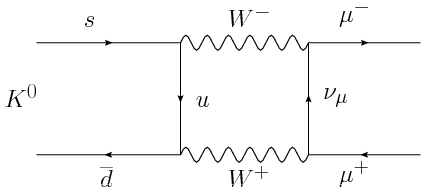
\includegraphics[width=0.5\textwidth]{Glashow-Illiopoulos-Maiani_mechanism_fig1.png}
	\caption{Box diagram describing $K_L^0\rightarrow\mu^-\mu^+$, through an intermediate $u$ quark. \Joao{A imagem tem pouca qualidade. Consegues fazer isto no latex com a package feynmp. No tutorial que te enviei tem lá o código}}
	\label{fig:Kaon}
\end{figure}

\Joaoout{We avoided discussing leptons since in the SM their mass eigenstates can be easily shown to have no real consequence besides a change of basis.} 
%
\Joaorep{You}{We} might also note a very interesting feature of the Standard Model, by consequence of the $\mathrm{SU(2)_L \times U(1)_Y }$ symmetry\Joaoadd{. T}here are no interactions of the right handed unitary matrices and \Joaorep{there for}{thus} no mixing, coupling, or charged currents of right handed quarks, making them theoretically invisible to measurements. \Joao{Já notei que às vezes usas ``you''. Não te dirigas para o arguente ou para que está a ler. Tenta usas sempre expressões com ``We''}
%
\begin{figure}[H]
	\centering
	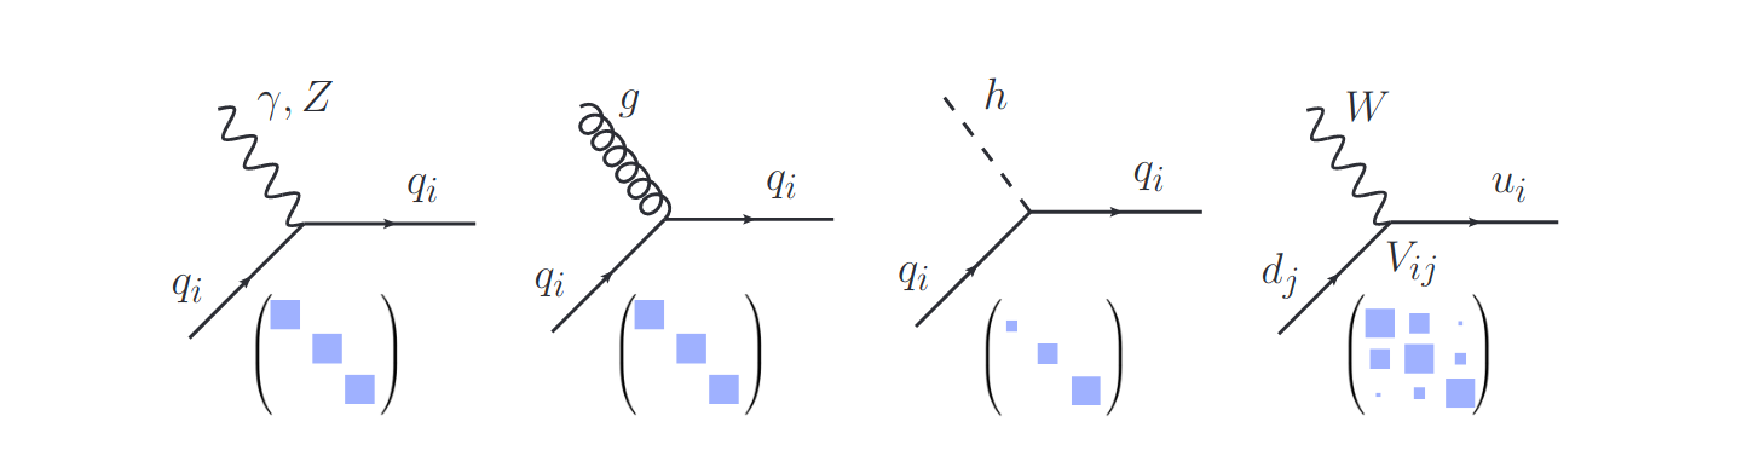
\includegraphics[width=0.9\textwidth]{TestYukawaCouplings.pdf}
	\caption{\Joaoout{The} Feynman diagrams for flavour conserving couplings of quarks to photon, $Z$ boson, gluon and the Higgs (the first three diagrams), and the flavour changing coupling to the $W$ (the last diagram). The $3\times3$ matrices are visual representations of couplings in the generation space, with couplings to $\gamma$, $Z$, $g$ \Joaoadd{being} flavour universal, \Joaorep{the}{while} couplings to the Higgs flavour \Joaoadd{are} diagonal but not universal\Joaorep{, and the couplings to}{. The couplings involving} $W$ \Joaoadd{are} flavour changing and hierarchical.}
	\label{fig:QuarkCKM}
\end{figure}
%

% Possible power gap
%
% Here we introduce the CKM matrix, a $3 \times 3$ unitary matrix. It is a paramatrization of the three mixing angles and CP-violating KM phase. There are many possible conventions to represent the CKM matrix. 

The CKM matrix elements are fundamental parameters of the particle physics, so their precise determination is important, and reproducing the quark mixing parameters is fundamental for BSM searches that include changes to how the quarks interact with possible new Higgs bosons. 
 

\subsection{Charged Flavour Currents vs. Neutral Flavor Currents}

It is very noteworthy to highlight a important distinction between flavor changing neutral and charged currents. FCNCs are processes in which the quark flavor changes, while the quark charge stays the same. 
%
The Flavour Changing Charged Currents (FCCCs) change both the flavour and the charge of the quark. 
%
Extracting some representative probabilities from \cite{Tanabashi2018} reveals that the two types of processes are strikingly statistically different.  
%
The charged currents lead to the dominant weak decays, while the FCNCs induce decays that are extremely suppressed. Rounding the experimental results, and not showing the errors, a few representative decays are, 
%
\setlength{\tabcolsep}{2pt} % Default value: 6pt
\renewcommand{\arraystretch}{1} % Default value: 1
%
\begin{table}[!htb]
    %\caption{Global caption}
    \begin{minipage}{.5\linewidth}
      \caption{FCCCs examples}
\centering
\begin{tabular}{lcl}
$s \rightarrow u \mu^- \nu_\mu $ & : & $\mathcal{BR}$ $\left( K^+ \rightarrow \mu^- \nu\right) = 64 \%$                 \\
$b \rightarrow c l^- \nu_l $       & : &  $\mathcal{BR}$ $\left( B^- \rightarrow D^0 l \overline{\nu}_l \right) = 2.3 \% $ \\
$c \rightarrow u \mu^- \nu_\mu $   & : &  $\mathcal{BR}$ $\left( D^\pm \rightarrow K^0 \mu^\pm \nu \right) = 9 \%$        
\end{tabular}
    \end{minipage}%
    \begin{minipage}{.5\linewidth}
      \centering
        \caption{FCNCs examples}
\begin{tabular}{lcl}
$s \rightarrow d \mu^+ \mu^- $ & : &  $\mathcal{BR}$ $\left( K_L \rightarrow\mu^+ \mu^- \right) =  7\times10^{-9}$        \\
$ b \rightarrow d \mu^+ \mu^-$ & : &  $\mathcal{BR}$ $\left( B^- \rightarrow  K^{\** -} l^+ l^- \right) =  5\times10^{-7}$ \\
$ c \rightarrow u l^+ l^-$     & : &  $\mathcal{BR}$ $\left( D^0 \rightarrow \pi l^+ l^- \right) =  1.8\times10^{-4}$      
\end{tabular}
    \end{minipage} 
\end{table}

\setlength{\tabcolsep}{6pt} % Default value: 6pt
\renewcommand{\arraystretch}{1} % Default value: 1

The reason for such a striking difference is that in the SM the charged currents occur at tree level, while FCNCs are forbidden at tree level and only arise starting at one loop order. Note the lack of neutral couplings (involving the $Z$ boson) between the up and down families in Eq \ref{LagFermFCCCs}. The relative complexity of these processes can be easily seen in Fig \ref{fig:Flavour_D_1},
%
\begin{figure}[H]
	\centering
	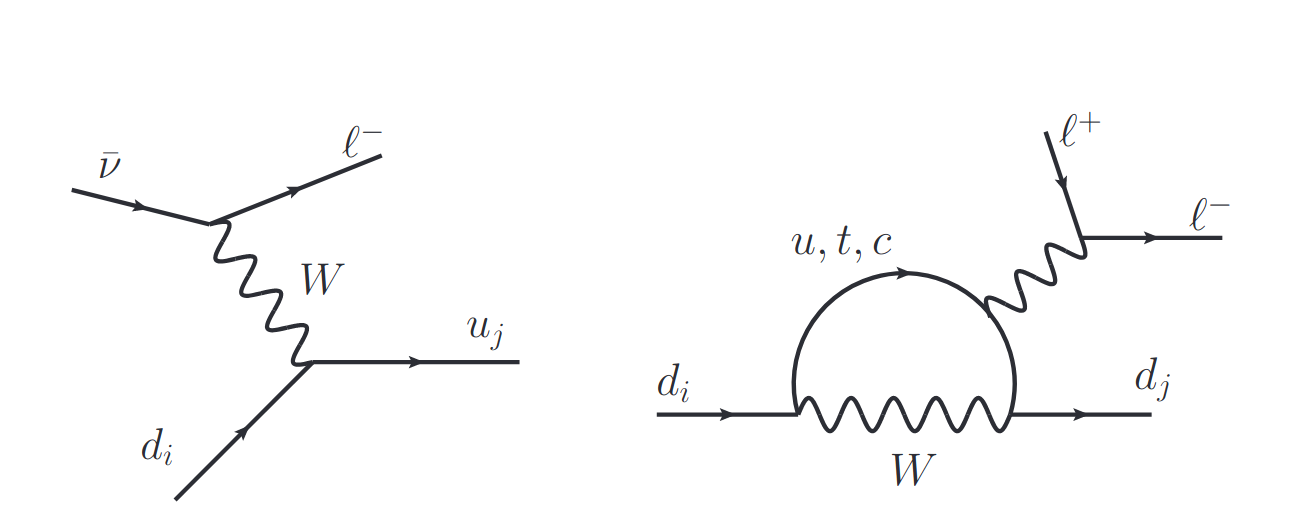
\includegraphics[width=0.75\textwidth]{Stolen.png}
	\caption{Representative tree level charged current diagram (left) and a loop induced FCNC diagram (right).}
	\label{fig:Flavour_D_1}
\end{figure}
%
%Making FCNCs virtual process.
%
Furthermore, the FCNCs come suppressed by the difference of the masses of the quarks running in the loop, $m^2_j-m^2_i$. This so called Glashow-Iliopoulos-Maiani (GIM) mechanism \cite{glashow1970weak}. Given the differences between the masses of the up and down sectors this has a significant impact. 
%
% A interesting result of this mechanism would be that that there is no flavour violation, if all the quark masses are the same. { \color{red} Relevant? }

\subsubsection{Flavour as a Probe into New Physics}

Now that we have introduced a small portion of flavor physics we can briefly touch on why collider experiments have been sold as a pathway to discovering new physics i.e. how deviation in rare decays could pin point exactly what is missing in the SM. 

Thanks to these large experiments we have many new observables in flavor physics, e.g. the branching ratios not coinciding with the SM prediction \cite{CasteloBranco2014}, observed Lepton Flavor Violation in tree and loop levels \cite{Graverini2019}.
%
As well as providing limits on processes that are prohibited in the SM but that could happen with different models, such as lepton flavor violation in Higgs decays \cite{Sirunyan_2018} in models without Lepton flavour universality. 
%
%For each of these examples there is also a plethora of different parent particles for each change of flavour, as well as many instances of final states. 
%
%The abundance of observables is clearly illustrated by opening the handy Particle Data Group (PDG) book \cite{Tanabashi2018}. 

However, one of the favored ways to search for NP is trough FCNCs this is because as mentioned there are no FCNCs at tree-level in the SM i.e. the gluon, Z and Higgs are strictly flavor conserving as we see in Fig.\,\ref{fig:QuarkCKM} at tree-level.  
%
Thus given FCNC processes are heavily suppressed in the SM trough the aforementioned GIM mechanism and loop order, and that FCNCs processes can be easily modified by NP, either through new tree level or loop level NP contributions these can serve as a good tool to search for exotic signatures. 
%
Note, these signatures could show themselves trough virtual NP particles and thus also provide evidence of high mass (Possibly TeV range) at a lower beam energy than the required energy to for one to be freely produced. 
%
This is if we assume NP can couple between generations and flavors of quarks. 

%Take the following example, if the $B_s$ meson mixing is affected by a NP process at tree-level the contribution of NP would be $\propto g^2_{sb} / M^2_{NP} $ where $g$ is the NP coupling to b and s quarks and $M_{NP}$ the mass of the new mediator.

%To shorten the discussion we will focus on the processes that are at present showing deviations from the SM expectations. 

The recipe then, seems simple, identify processes that are rare in the SM and then search for deviations from the SM predictions.
%
However, thus far all but a few processes are within $2\sigma$ experimental and theoretical bounds given by the SM. 
%
Some of the most radical being the quark level transitions, $b \rightarrow s \mu \mu$ \cite{DAmico2017}%,Geng_2017} 
 and $b \rightarrow c \tau \nu$ \cite{Hu2019} channels. %\footnote{There are other interesting ones like the $\dfrac{\epsilon^\prime}{\epsilon}$ ratio, but not quite as large \cite{Buras2015}} \cite{Fajfer_2012}
%
They are, so far, showing over $ 4 \sigma$ deviations from their expected value. 
%{\color{blue} there are very bold claims I need to better cite my work (citation needed)}.

Without going into too much depth onto the NP searches, we can examine the scale at which these processes are "integrated away". 
%
This is the energy scale at which a NP operator would allow these processes to exist only at high energies. These energies are naturally high given the terms in Eq.\,(\ref{eq:NP}). 
% Avoiding going in depth into these processes, what this might point us too, by these processes as suppressed the vector-axial processes. For them to be integrated away we get very different, but high, energy scales. There would have to exist terms a kin to, 
%If examined through V-A operators the NP scale of these 2 processes are both very different and very heavy, these would be something a kin to, 
%
\bigbreak
%
\noindent\begin{minipage}{.35\textwidth}
	\begin{figure}[H]
		\label{fig:contactNP}
		\centering
		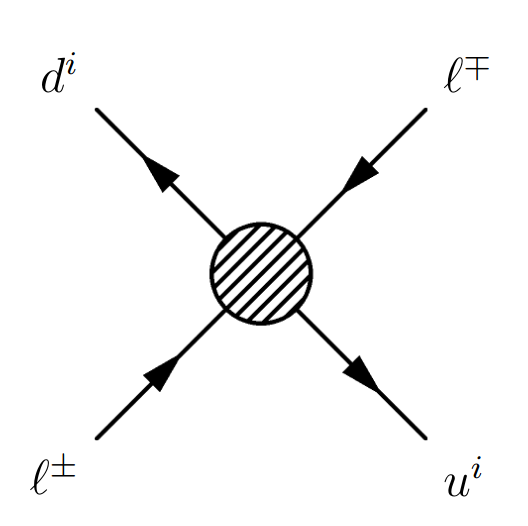
\includegraphics[width=0.6\textwidth]{My_First_Diagram.png}
		\caption{"Contact" interactions with loop interactions containing NP}
	\end{figure}
\end{minipage}
\begin{minipage}{.6\textwidth}
\begin{equation}
\label{eq:NP}
\mathcal{L}_{NP} \supset \frac{1}{\Lambda_{NP}} (\overline{Q}_i \gamma^\mu \sigma Q_j ) (\overline{L}_k \gamma_\mu \sigma L_l) ,  
\end{equation}
\end{minipage}
%
\bigbreak
%
To explain $b \rightarrow s \mu \mu$ transitions you would need a $\Lambda_{NP} \approx 3 \ \text{TeV}$ while for $b \rightarrow c \tau \nu$ you would need a $\Lambda_{NP} \approx 30\ \text{TeV}$. This is a strong indicator that some components are missing in our formulation like a new mediator for gauge interactions. The advantage of this scale is it lies almost certainly in most BSM scenarios, avoiding most experimental constraints.

As for the FCNC diagram, the $b \rightarrow s \mu \mu$ channel can be seen in Fig \ref{fig:Flavour_D_2_Muon}, 
%
\begin{figure}[H]
	\centering
	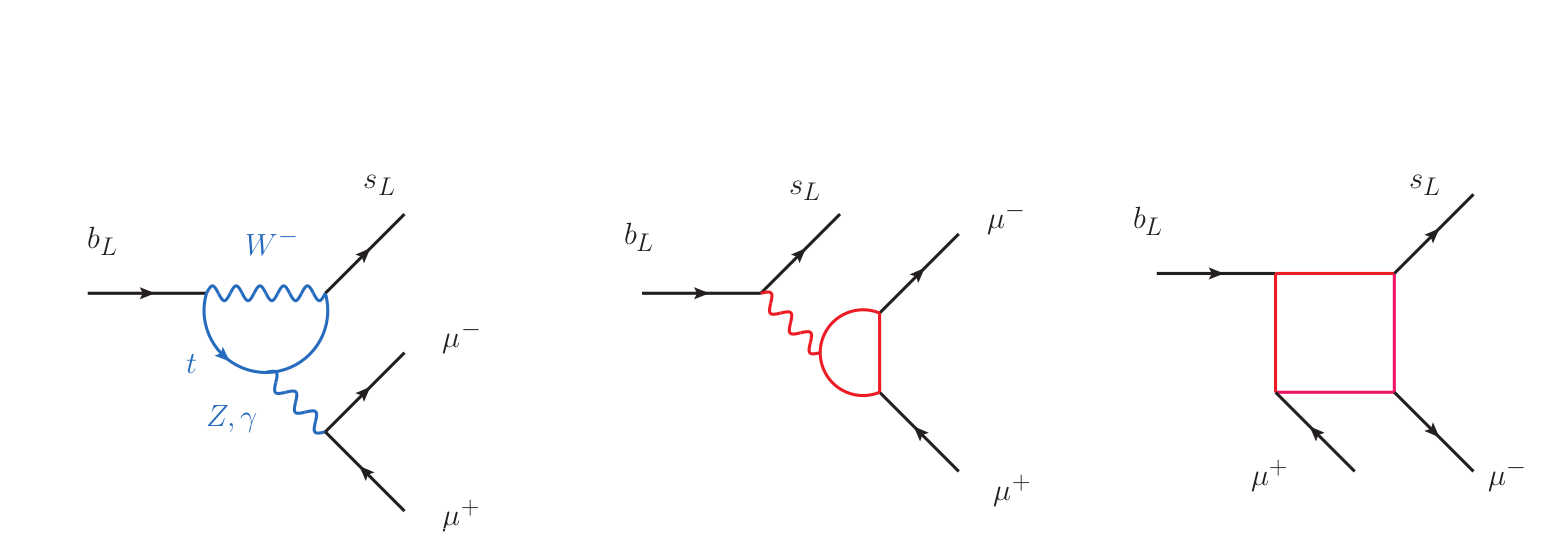
\includegraphics[width=0.95\textwidth]{Stolen_2.png}
	\caption{A representative SM diagram for $b \rightarrow s \mu \mu$ transition (left), and representative possible loop level NP
contributions (middle and right).}
	\label{fig:Flavour_D_2_Muon}
\end{figure}
%
The $b \rightarrow c \tau \nu$ flavour anomaly is similarly very clean theoretically \cite{Fajfer_2012}. However, the NP effect in these diagrams is large ($\mathcal{O}(20\%)$) compared to the SM. This means that the scale of NP needs to be lower or happen at tree-level. Consequently the NP interpretations here are often in conflict with experimental constraints, such as this decay.
%
The theoretical bias here would have been that the new charged currents are either due to a charged Higgs, $H^+$ , or a new vector boson, $W^\prime$, see Fig. \ref{fig:Flavour_D_3_Tau}. However these would have too large a effect in the $B^-$ lifetime to fully explain the anomaly according to Ref.\,\cite{Alonso_2017}.
%
\begin{figure}[H]	
	\centering
	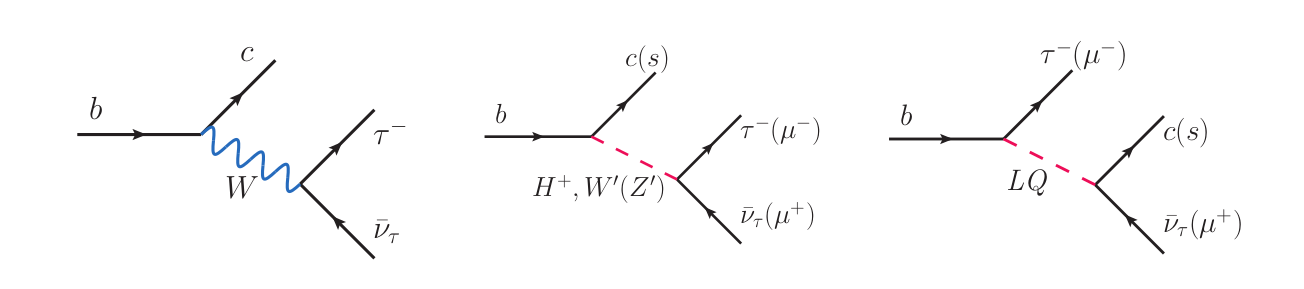
\includegraphics[width=0.95\textwidth]{Stolen_3.png}
	\caption{The SM diagrams for $b \rightarrow c \tau \nu$ transition (left), and the possible tree level NP contributions to $b \rightarrow c \tau \nu$ transition (middle and right). Where the LQ stands for a hypothetical Leptoquark particle that would interact with both leptons and quarks.}
	\label{fig:Flavour_D_3_Tau}
\end{figure}
%
Another prediction of the SM is that the rates for the  $b \rightarrow s e^+ e^-$ and  $b \rightarrow s \mu^- \mu^+$ transitions should be equal to each other.
%
The SM prediction of Lepton Flavour Universality (LFU) is deeply engrained in the structure of the theory, since it is a consequence of the fact that the electroweak gauge group is the same for all three generations. 
%
The prediction of LFU can be tested experimentally, also trough flavour physics, by theoretically clean observables such as the ratios of these flavour observables, 
%
\begin{equation}
R_{K^{\**}} = \frac{\text{Br}( B \rightarrow K^{\**} \mu^- \mu^+ )}{\text{Br} (  B \rightarrow K^{\**} e^- e^+  )} ,
\end{equation}
% 
Another strong indicator of new physics is the fact the experimental value for this ratio is $R_{K^{\**}} \approx 0.7$, violating LFU by $2.2 - 2.6 \sigma$ \cite{Wei_2009}. Revealing to yet another discrepancy between the SM and reality. 

%\subsubsection{The Future of Flavour Indirect Searches}
%
%The NP searches with rare decays, will benefit from the upcoming upgrades at Belle II and the LHC. Belle II expects to collect 50 times the Belle dataset.
%
%While for the LHC, after upgrade II aims for roughly 100 times the present data set with an upgraded detector. {\color{blue} (citation needed)}.
%
%Undoubtedly this improvement in sensibility will translate to a finer value for all measurable parameters at these experiments. We expect these anomalies then to go over the required $5 \sigma$ in future experiments (Assuming of course, they are not statistical deviations).
%
%We expect progress in leptonic decays to finally start excluding large portions of the parameter space of several models. 
%
%{ \color{red} Ask Morais: Should I add more? or remove? }

